%
% This document contains the chapter about AC noise analysis.
%
% Copyright (C) 2005 Stefan Jahn <stefan@lkcc.org>
% Copyright (C) 2005 Michael Margraf <Michael.Margraf@alumni.TU-Berlin.DE>
%
% Permission is granted to copy, distribute and/or modify this document
% under the terms of the GNU Free Documentation License, Version 1.1
% or any later version published by the Free Software Foundation.
%

\chapter{AC Noise Analysis}
%\addcontentsline{toc}{chapter}{AC Noise Analysis}

\section{Definitions}
%\addcontentsline{toc}{section}{Definitions}

First some definition must be done:

\addvspace{12pt}

\emph{Reciprocal Networks:}\\
Two networks $A$ and $B$ are reciprocal to each other if their
transimpedances have the following relation:
\begin{equation}
Z_{mn,A} = Z_{nm,B}
\end{equation}

That means: Drive the current $I$ into node $n$ of circuit $A$ and
at node $m$ the voltage $I\cdot Z_{mn,A}$ appears. In circuit $B$
it is just the way around.

\addvspace{12pt}

\emph{Adjoint Networks:}\\
Network $A$ and network $B$ are adjoint to each other if the following
equation holds for their MNA matrices:
\begin{equation}
[A]^T = [B]
\end{equation}

\section{The Algorithm}
%\addcontentsline{toc}{section}{The Algorithm}

To calculate the small signal noise of a circuit, the AC noise
analysis has to be applied \cite{Blum}.  This technique uses the
principle of the AC analysis described in chapter \ref{sec:acMNA} on
page \pageref{sec:acMNA}.  In addition to the MNA matrix $A$ one needs
the noise current correlation matrix $\underline{C}_Y$ of the circuit,
that contains the equivalent noise current sources for every node on
its main diagonal and their correlation on the other positions.

\addvspace{12pt}

The basic concept of the AC noise analysis is as follows: The
noise voltage at node $i$ should be calculated, so the voltage arising
due to the noise source at node $j$ is calculated first. This has to
be done for every $n$ nodes and after that adding all the noise
voltages (by paying attention to their correlation) leads to the
overall voltage. But that would mean to solve the MNA equation $n$
times.  Fortunately there is a more easy way.  One can perform the
above-mentioned $n$ steps in one single step, if the reciprocal MNA
matrix is used. This matrix equals the MNA matrix itself, if the
network is reciprocal.  A network that only contains resistors,
capacitors, inductors, gyrators and transformers is reciprocal.

\addvspace{12pt}

The question that needs to be answered now is: How to get the
reciprocal MNA matrix for an arbitrary network? This is equivalent to
the question: How to get the MNA matrix of the adjoint network.
The answer is quite simple: Just transpose the MNA matrix!

\addvspace{12pt}

For any network, calculating the noise voltage at node $i$ is done by
the following three steps:
\begin{alignat}{2}
 & \textrm{1. Solving MNA equation:} & \qquad & \left[A\right]^T \cdot \left[x\right] =
\left[A\right]^T \cdot
\begin{bmatrix}
v \\
j \\
\end{bmatrix}
=
\begin{bmatrix}
0 \\
\vdots \\
0 \\
-1 \\
0 \\
\vdots \\
0 \\
\end{bmatrix}
\leftarrow i\textrm{-th row} \\
 & \textrm{2. Creating noise correlation matrix:} & \qquad
 & \left( \underline{C}_Y \right) \\
 & \textrm{3. Calculating noise voltage:} & \qquad
 & v_{noise,i} = \sqrt{\left[v\right]^T \cdot \left( \underline{C}_Y \right) \cdot \left[v\right]^*}
\end{alignat}

If the normal AC analysis has already be done with LU decomposition,
then the most time consuming work of step 1 has already be done.
\begin{equation}
\textrm{instead of} \qquad Y = L\cdot U \qquad \textrm{we have} \qquad
Y^T = U^T \cdot L^T
\end{equation}

I.e. $U^T$ becomes the new $L$ matrix and $L^T$ becomes the new $U$
matrix, and the matrix equation do not need to be solved again, because
only the right-hand side was changed.  So altogether this is a quickly
done task.  (Note that in step 3, only the subvector $[v]$ of vector
$[x]$ is used.  See section \ref{sec:xmatrix} for details on this.)

\addvspace{12pt}

If the noise voltage at another node needs to be known, only the
right-hand side of step 1 changes.  That is, a new LU decomposition is
not needed.

\addvspace{12pt}

Reusing the LU decomposed MNA matrix of the usual AC analysis is
possible if there has been no pivoting necessary during the
decomposition.

\addvspace{12pt}

When using either Crout's or Doolittle's definition of the LU
decomposition during the AC analysis the decomposition representation
changes during the AC noise analysis as the matrix $A$ gets
transposed.  This means:
\begin{equation}
A = L\cdot U \;\text{ with }\;
L = 
\begin{bmatrix}
l_{11} & 0 & \ldots & 0\\
l_{21} & l_{22} & \ddots & \vdots\\
\vdots &  & \ddots & 0\\
l_{n1} & \ldots & \ldots & l_{nn}
\end{bmatrix}
\;\text{ and }\;
U =
\begin{bmatrix}
1 & u_{12} & \ldots & u_{1n}\\
0 & 1 &  & \vdots\\
\vdots & \ddots & \ddots & \vdots\\
0 & \ldots & 0 & 1
\end{bmatrix}
\end{equation}

becomes
\begin{equation}
A^T = U^T\cdot L^T \;\text{ with }\;
L = 
\begin{bmatrix}
1 & 0 & \ldots & 0\\
l_{21} & 1 & \ddots & \vdots\\
\vdots &  & \ddots & 0\\
l_{n1} & \ldots & \ldots & 1
\end{bmatrix}
\;\text{ and }\;
U =
\begin{bmatrix}
u_{11} & u_{12} & \ldots & u_{1n}\\
0 & u_{22} &  & \vdots\\
\vdots & \ddots & \ddots & \vdots\\
0 & \ldots & 0 & u_{nn}
\end{bmatrix}
\end{equation}

Thus the forward substitution (as described in section
\ref{sec:CroutFSubst}) and the backward substitution (as described in
section \ref{sec:CroutBSubst}) must be slightly modified.
\begin{align}
y_{i} &= z_{i} - \sum_{k=1}^{i-1} y_{k}\cdot l_{ik} & i = 1,\ldots,n
\end{align}
\begin{align}
x_{i} &= \frac{y_{i}}{u_{ii}} - \sum_{k=i+1}^{n} x_{k}\cdot \frac{u_{ik}}{u_{ii}} & i = n,\ldots,1
\end{align}

Now the diagonal elements $l_{ii}$ can be neglected in the forward
substitution but the $u_{ii}$ elements must be considered in the
backward substitution.

\subsection{A Simple Example}
%\addcontentsline{toc}{subsection}{A Simple Example}

The network that is depicted in figure \ref{fig:mna_noise1} is given.
The MNA equation is (see chapter \ref{sec:MNA}):
\begin{equation}
[A]\cdot [x] =
\begin{bmatrix}
1/R_1 & 0\\
  G   & 1/R_2
\end{bmatrix}
\cdot
\begin{bmatrix}
V_1\\
V_2
\end{bmatrix}
=
\begin{bmatrix}
0\\
0
\end{bmatrix}
\end{equation}

\begin{figure}[ht]
\begin{center}
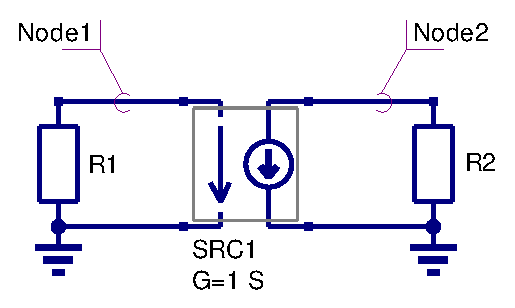
\includegraphics[width=7cm]{MNAnoise1}
\end{center}
\caption{simple non-reciprocal network}
\label{fig:mna_noise1}
\end{figure}
\FloatBarrier

Because of the controlled current source, the circuit is not
reciprocal.  The noise voltage at node 2 the one to search for.  Yes, this
is very easy to calculate, because it is a simple example, but
the algorithm described above should be used.  This can be achived
by solving the equations
\begin{equation}
\begin{bmatrix}
1/R_1 & 0\\
  G   & 1/R_2
\end{bmatrix}
\cdot
\begin{bmatrix}
Z_{11}\\
Z_{21}
\end{bmatrix}
=
\begin{bmatrix}
-1\\
0
\end{bmatrix}
\end{equation}
and
\begin{equation}
\begin{bmatrix}
1/R_1 & 0\\
  G   & 1/R_2
\end{bmatrix}
\cdot
\begin{bmatrix}
Z_{12}\\
Z_{22}
\end{bmatrix}
=
\begin{bmatrix}
0\\
-1
\end{bmatrix}
\end{equation}
So, the MNA matrix must be solved two times: First to get the
transimpedance from node 1 to node 2 (i.e. $Z_{21}$) and second to get
the transimpedance from node 2 to node 2 (i.e.  $Z_{22}$).  But why
solving it two times, if only one voltage should be calculated? With every
step transimpedances are calculated that are not need.  Is there no more
effective way?

\addvspace{12pt}

Fortunately, there is Tellegen's Theorem: A network and its adjoint
network are reciprocal to each other.  That is, transposing
the MNA matrix leads to the one of the reciprocal
network.  To check it out:

\begin{equation}
[A]^T\cdot [x] =
\begin{bmatrix}
1/R_1 & G\\
  0   & 1/R_2
\end{bmatrix}
\cdot
\begin{bmatrix}
V_1\\
V_2
\end{bmatrix}
=
\begin{bmatrix}
0\\
0
\end{bmatrix}
\end{equation}

\begin{figure}[ht]
\begin{center}
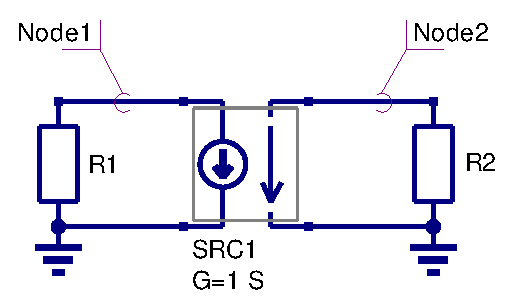
\includegraphics[width=7cm]{MNAnoise2}
\end{center}
\caption{simple network to compare with adjoint network}
\label{fig:mna_noise2}
\end{figure}
\FloatBarrier

Compare the transposed matrix with the reciprocal network in figure
\ref{fig:mna_noise2}.  It is true!  But now it is:
\begin{equation}
\begin{bmatrix}
1/R_1 & G\\ 0 & 1/R_2
\end{bmatrix}
\cdot
\begin{bmatrix}
Z_{12,reciprocal}\\
Z_{22,reciprocal}
\end{bmatrix}
=
\begin{bmatrix}
1/R_1 & G\\
  0   & 1/R_2
\end{bmatrix}
\cdot
\begin{bmatrix}
Z_{21}\\
Z_{22}
\end{bmatrix}
=
\begin{bmatrix}
0\\
-1
\end{bmatrix}
\end{equation}

Because $Z_{21}$ of the original network equals $Z_{12}$ of the
reciprocal network, the one step delivers exactly what is needed.
So the next step is:
\begin{equation}
([A]^T)^{-1}\cdot
\begin{bmatrix}
  0\\
 -1
\end{bmatrix}
=
\begin{bmatrix}
R_1 & -G\cdot R_1\cdot R_2\\
  0 & R2
\end{bmatrix}
\cdot
\begin{bmatrix}
  0\\
 -1
\end{bmatrix}
=
\begin{bmatrix}
G\cdot R_1\cdot R_2\\
-R_2
\end{bmatrix}
=
\begin{bmatrix}
Z_{21}\\
Z_{22}
\end{bmatrix}
\end{equation}

Now, as the transimpedances are known, the noise voltage
at node 2 can be computed. As there is no correlation, it writes
as follows:
\begin{eqnarray}
<v_{node2}^2> & = & <v_{R1,node2}^2> + <v_{R2,node2}^2> \\
  & = & <i_{R1}^2>\cdot Z_{21}\cdot Z_{21}^* + <i_{R2}^2>\cdot Z_{22}\cdot Z_{22}^* \\
  & = & \frac{4\cdot k\cdot T\cdot \Delta f}{R_1} \cdot (G\cdot R_1\cdot R_2)^2 +
        \frac{4\cdot k\cdot T\cdot \Delta f}{R_2} \cdot (-R_2)^2 \\
  & = & 4\cdot k\cdot T\cdot \Delta f\cdot \left( R_1\cdot (G\cdot R_2)^2 + R_2 \right)
\end{eqnarray}

That's it. Yes, this could have be computed more easily, but now
the universal algorithm is also clear.

\section{Noise Current Correlation Matrix}
%\addcontentsline{toc}{section}{Noise Current Correlation Matrix}

This section describes the noise current correlation matrices of noisy
components.  The equations are built for RMS noise currents with
$1\hertz$ bandwidth.

\subsection{Resistor}
%\addcontentsline{toc}{subsection}{Resistor}

Resistor with resistance $R$ and temperature $T$:
\begin{equation}
(\underline{C}_Y) = \frac{4\cdot k\cdot T}{R} \cdot
\begin{pmatrix}
 1 & -1 \\
-1 &  1 \\
\end{pmatrix}
\end{equation}

\subsection{Noise current source}
%\addcontentsline{toc}{subsection}{Noise current source}

Noise current source with a current power spectral density of $cPSD$:
\begin{equation}
(\underline{C}_Y) = cPSD \cdot
\begin{pmatrix}
 1 & -1 \\
-1 &  1 \\
\end{pmatrix}
\end{equation}

\subsection{Noise voltage source}
%\addcontentsline{toc}{subsection}{Noise voltage source}

A noise voltage source (voltage power spectral density $vPSD$) cannot
be modeled with the noise current matrix.  That is why one has to use
a noise current source (current power spectral density $cPSD$)
connected to a gyrator (transimpedance $R$) satisfying the equation
\begin{equation}
vPSD = cPSD \cdot R
\end{equation}

Figure \ref{fig:Unoise} shows an example.
\begin{figure}[ht]
\begin{center}
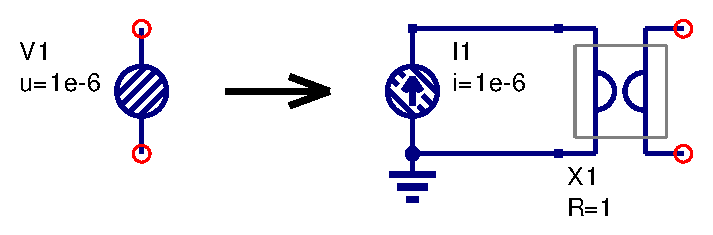
\includegraphics[width=9cm]{Unoise}
\end{center}
\caption{noise voltage source (left-hand side) and its equivalent circuit (right-hand side)}
\label{fig:Unoise}
\end{figure}
\FloatBarrier

The MNA matrix entries of the above construct (gyrator ratio $R=1$) is
similiar to a voltage source with zero voltage.
\begin{equation}
\begin{bmatrix}
.&.& -1\\
.&.& 1\\
1 & -1 & 0
\end{bmatrix}
\cdot
\begin{bmatrix}
V_{1}\\
V_{2}\\
I_x
\end{bmatrix}
=
\begin{bmatrix}
I_{1}\\
I_{2}\\
0
\end{bmatrix}
\end{equation}

The appropriate noise current correlation matrix yields:
\begin{equation}
(\underline{C}_Y) = cPSD \cdot
\begin{pmatrix}
 0 & 0 & 0\\
 0 & 0 & 0\\
 0 & 0 & 1\\
\end{pmatrix}
\end{equation}

\subsection{Attenuator}
%\addcontentsline{toc}{subsection}{Attenuator}

Attenuator with (power) attenuation $L$, reference impedance $Z_{ref}$
and temperature $T$:
\begin{equation}
(\underline{C}_Y) = 4\cdot k\cdot T\cdot \textrm{Re}\left(\underline{Y}\right)
 = \frac{4\cdot k\cdot T}{Z_{ref}\cdot (L-1)} \cdot
\begin{pmatrix}
 L+1            & -2\cdot\sqrt{L} \\
-2\cdot\sqrt{L} &  L+1 \\
\end{pmatrix}
\end{equation}

\subsection{Isolator}
%\addcontentsline{toc}{subsection}{Isolator}

Isolator with reference impedance $Z_1$ (input) and $Z_2$ (output) and
temperature $T$:
\begin{equation}
(\underline{C}_Y) = 4\cdot k\cdot T\cdot
\begin{pmatrix}
 1/Z_1                 & 0 \\
-2/\sqrt{Z_1\cdot Z_2} &  1/Z_2 \\
\end{pmatrix}
\end{equation}

\subsection{Diode}
%\addcontentsline{toc}{subsection}{Diode}

Diode (for details on the parameters see section \ref{sec:nw_diode}):
\begin{equation}
(\underline{C}_Y)
 = 2\cdot e\cdot K\cdot \left(I_{d} + 2\cdot I_{S}\right)\cdot
\begin{pmatrix}
   1 & -1\\
  -1 &  1\\
\end{pmatrix}\\
\end{equation}
